\documentclass[../main.tex]{subfiles}

\begin{document}

\section{Handling multiple testing problem through effect calibration: implementation using PyMC}
\authors{%
Lea Waller\textsuperscript{1}, %
Kelly Garner\textsuperscript{2}, %
Christopher R Nolan\textsuperscript{3}, %
Daniel Borek\textsuperscript{4}, %
Gang Chen\textsuperscript{5}\\
}
\affiliations{%
\noindent1. Charité Universitätsmedizin Berlin, corporate member of Freie Universität Berlin and Humboldt-Universität zu Berlin, Department of Psychiatry and Neurosciences CCM, Berlin, Germany\\ %
2. School of Psychology, The University of Queensland, St. Lucia, 4072, QLD, Australia\\ %
3. School of Psychology, The University of New South Wales, NSW, Australia\\ %
4. Department of Data Analysis, Faculty of Psychology and Educational Sciences, Ghent University, Ghent, Belgium\\ %
5. Scientific and Statistical Computing Core, NIMH, NIH, Department of Health and Human Services, USA %
}

\subsection{Introduction}

Human brain imaging data is massively multidimensional, yet current approaches to modelling functional brain responses entail the application of univariate inferences to each voxel separately. This leads to the multiple testing problem and unrealistic assumptions about the data such as artificial dichotomization (statistically significant or not) in result reporting. The traditional approach of massively univariate analysis assumes that no information is shared across the brain, effectively making a strong prior assumption of a uniform distribution of effect sizes, which is unrealistic given the connectivity of the human brain. The consequent requirement for multiple testing adjustments results in the \textit{calibration of statistical evidence} without considering the estimation of effect, leading to substantial information loss and an unnecessarily heavy penalty.

A more efficient approach to handling multiplicity focuses on the \textit{calibration of effect estimation} under a Bayesian multilevel modeling framework with a prior assumption of, for example, normality across space \parencite{chenHandlingMultiplicityNeuroimaging2019}. The methodology has previously been implemented at the region level into the \texttt{AFNI} program \texttt{RBA} \parencite{chen_sources_2022} using \texttt{Stan} through the \texttt{R} package \texttt{brms} \parencite{burknerBrmsPackageBayesian2017}. We intend to achieve two goals in this project: 
\begin{enumerate}[label=(\roman*),nolistsep]
    \item To re-implement the methodology using PyMC improve the performance and flexibility of the modeling approach.
    \item To explore the possibility of analyzing voxel-level data using the multilevel modeling approach
\end{enumerate}

\begin{figure*}[t!]
\centering
\begin{subfigure}{.5\textwidth}
    \centering
    \caption{Posterior distributions: \texttt{brms}}
    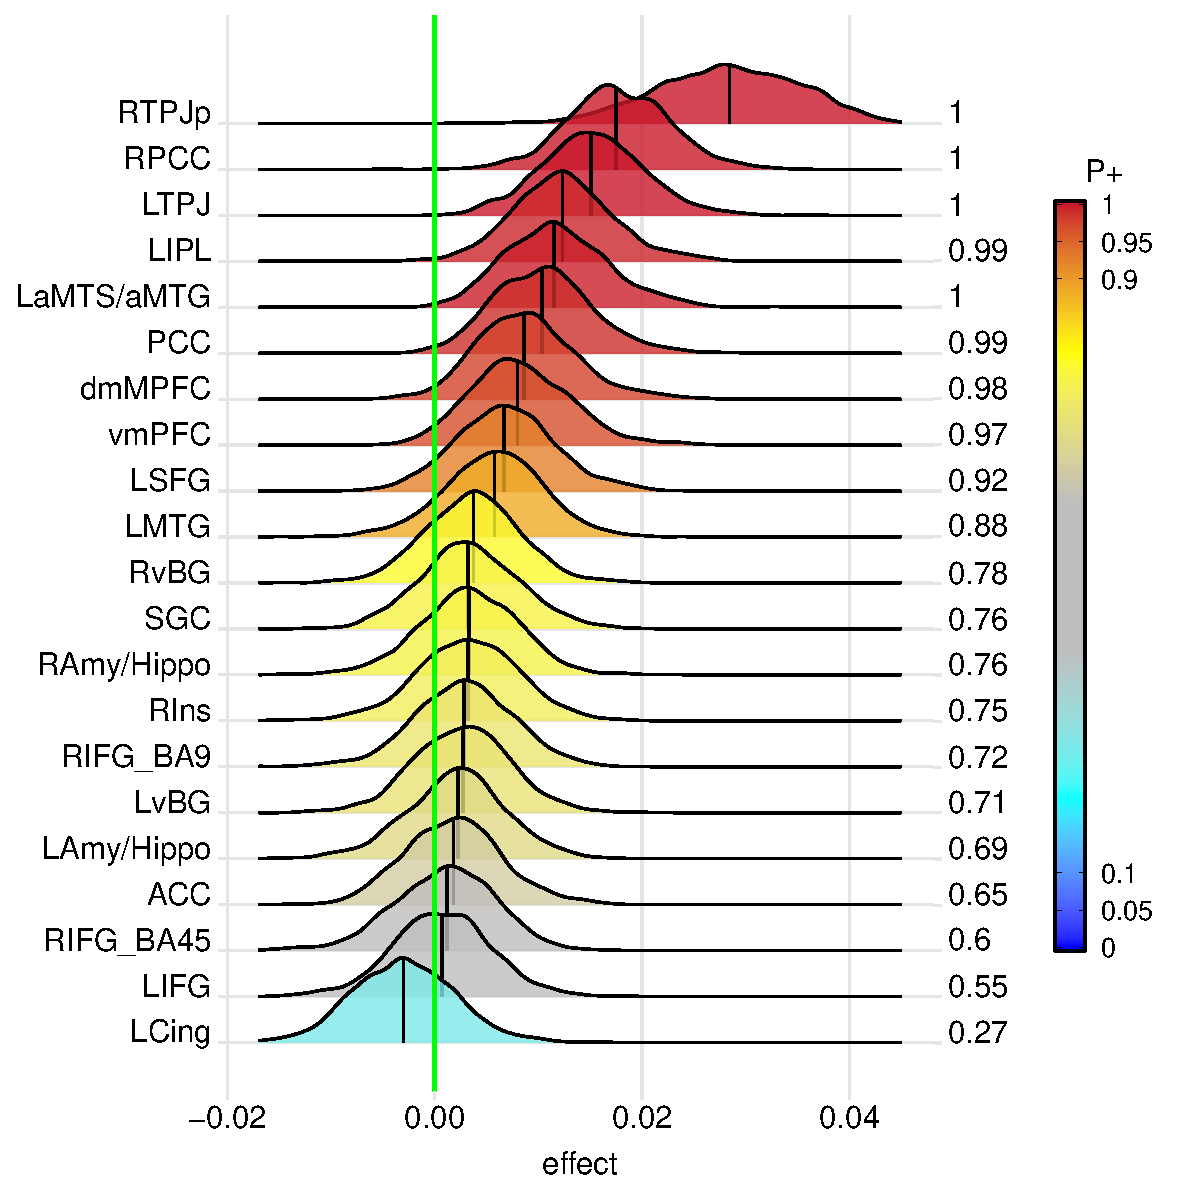
\includegraphics[width=.925\linewidth]{rba_brms.pdf}
    \label{fig:sub1}
\end{subfigure}%
\begin{subfigure}{.5\textwidth}
    \centering
    \caption{Posterior distributions: PyMC}
    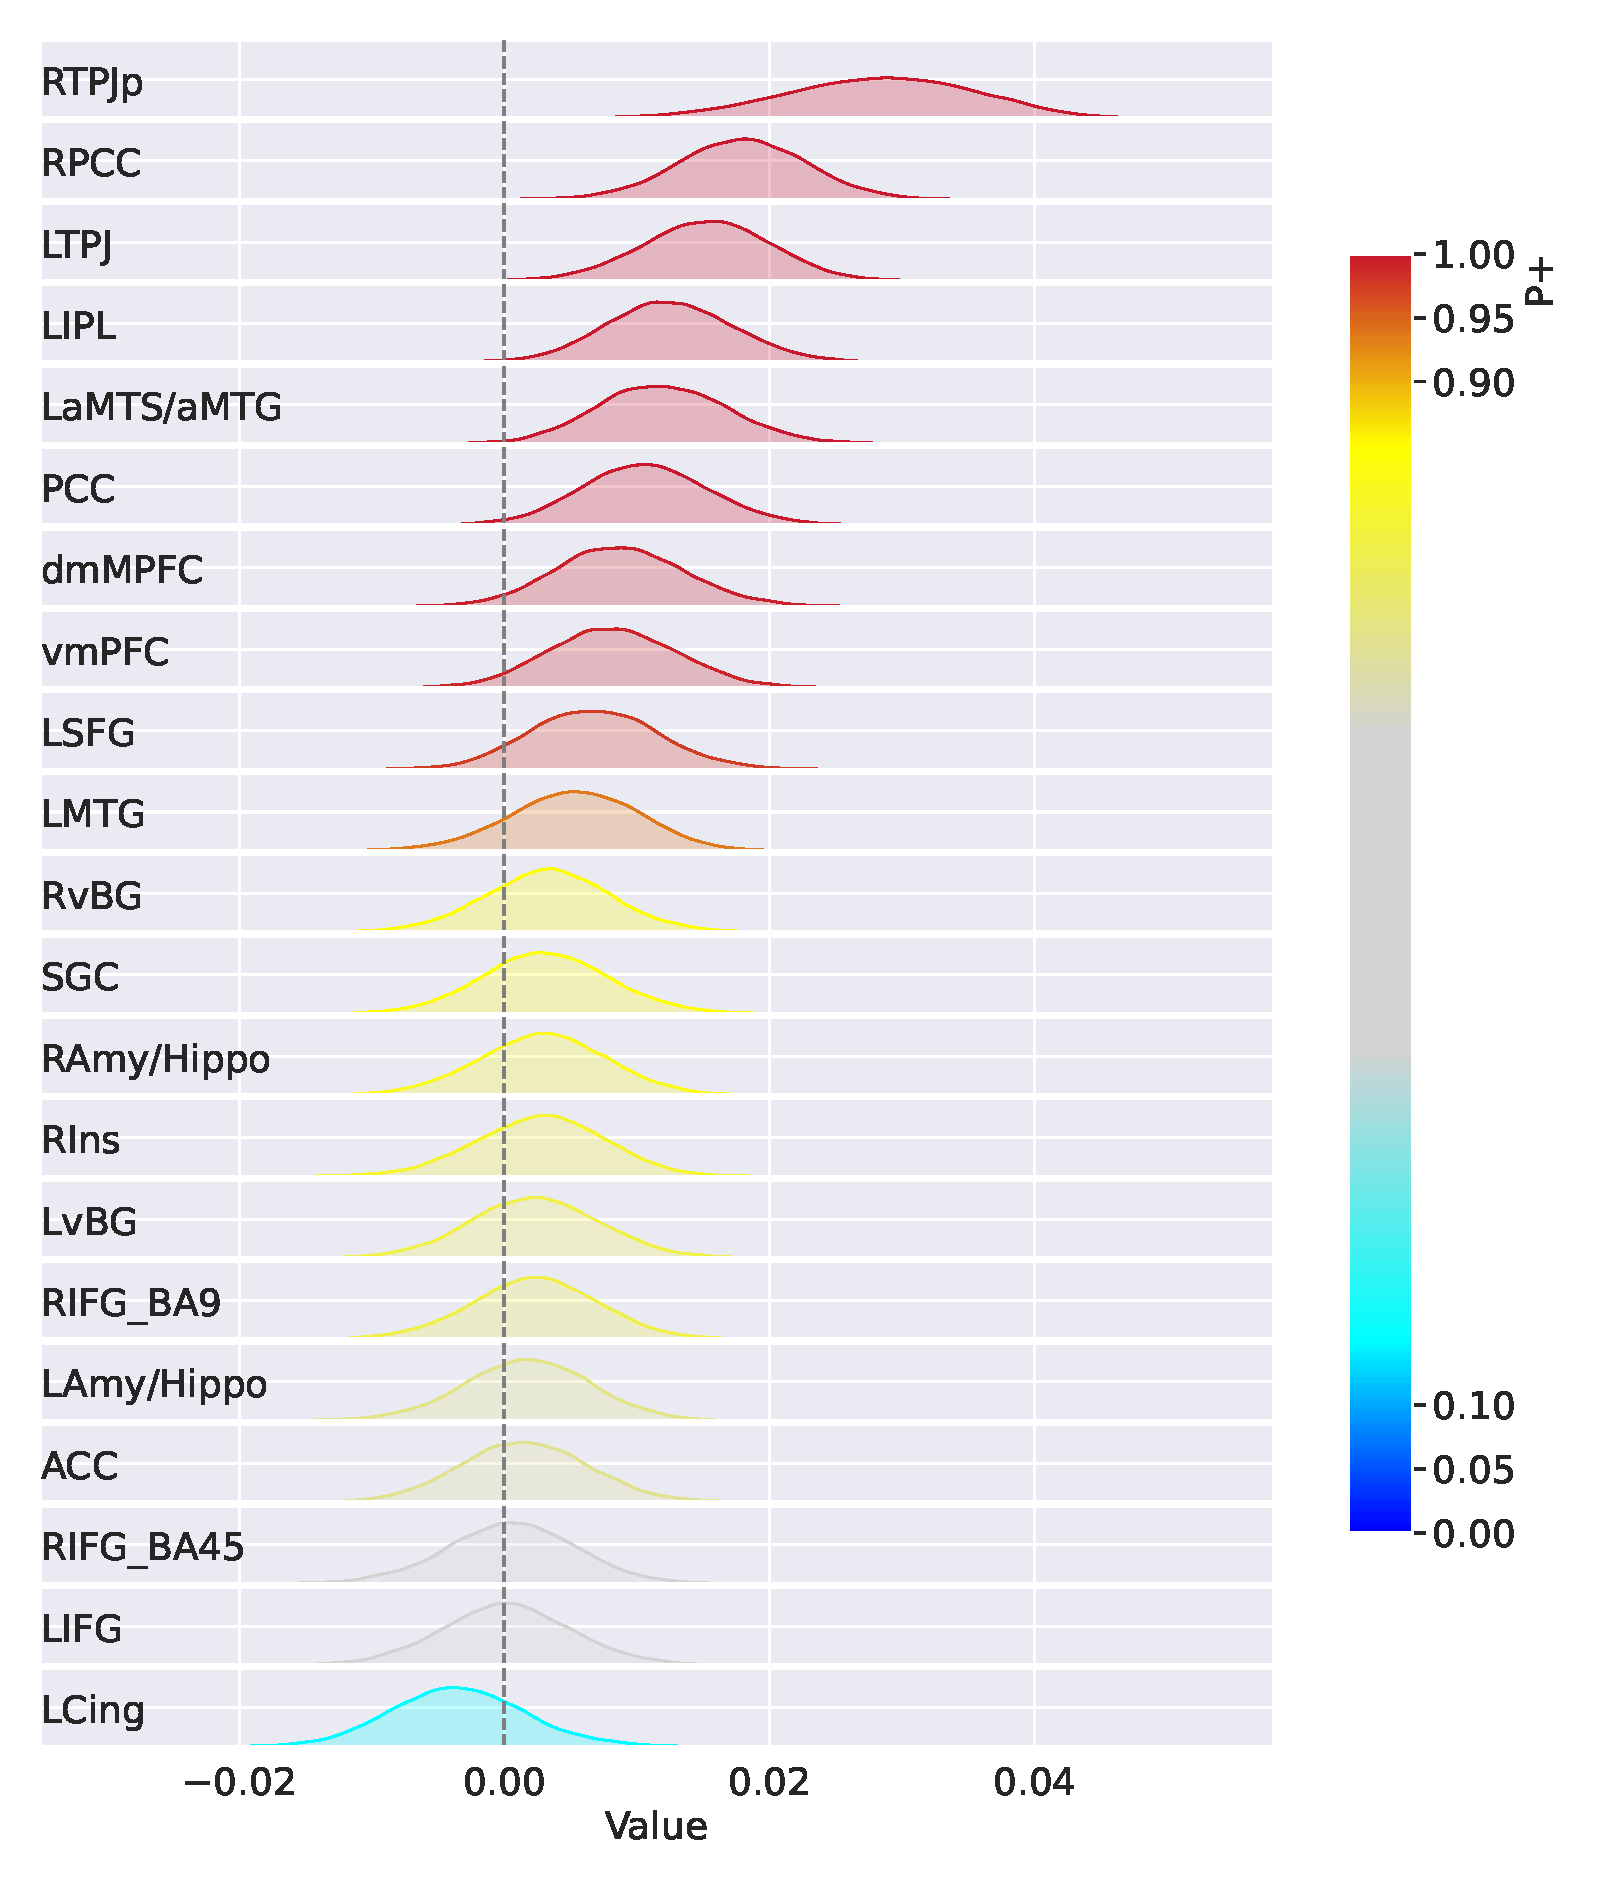
\includegraphics[width=.8\linewidth]{rba_bambi_pymc.pdf}
    \label{fig:sub2}
\end{subfigure}
\begin{subfigure}{.9\textwidth}
    \centering
    \caption{Extension to voxel-level analysis. }
    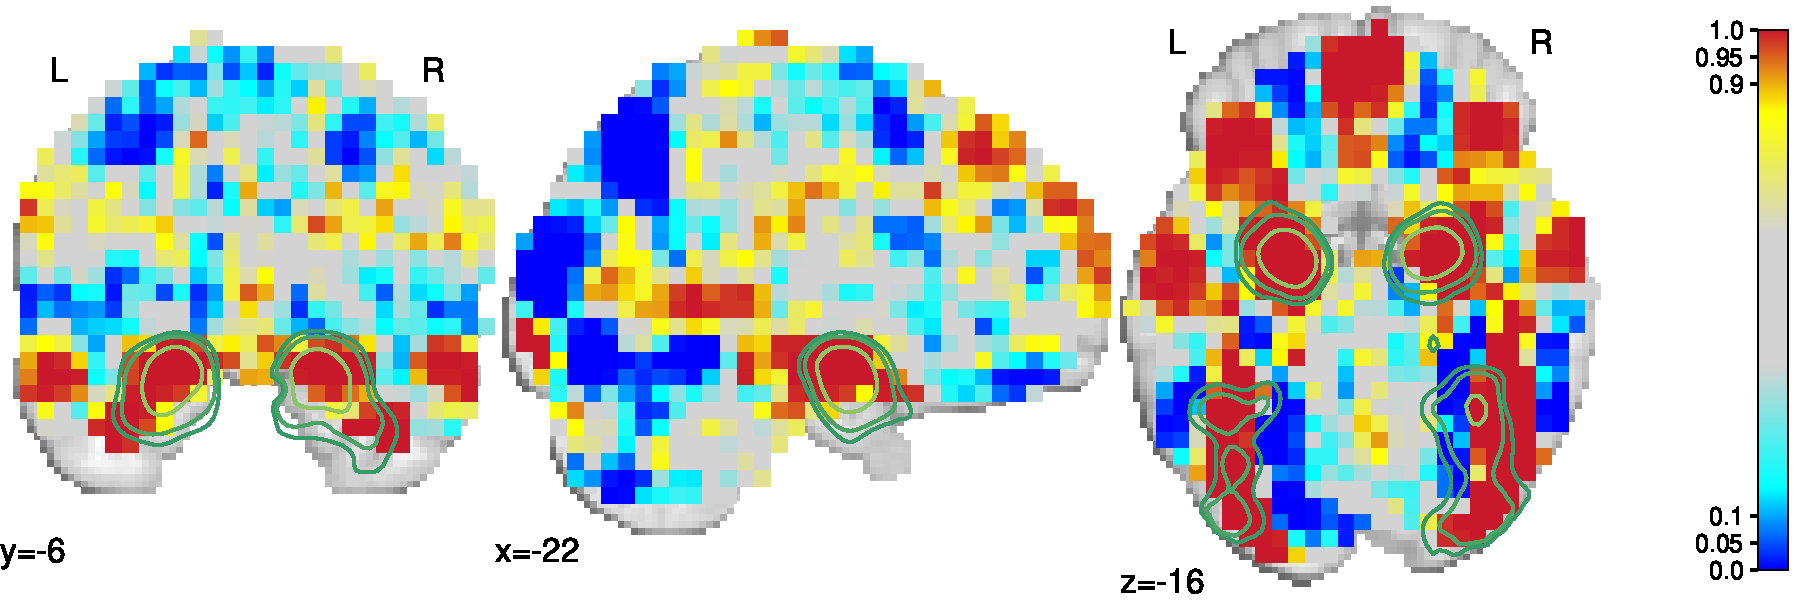
\includegraphics[width=.9\linewidth]{rba_voxel_level.pdf}
    \label{fig:vox}
\end{subfigure}

\caption{Validation of implementation using PyMC. (A) Posterior distributions of region-level behavior effects using \texttt{brms}. (B) Posterior distributions of region-level behavior effects using PyMC. (C) Posterior probabilities of the voxel-level effects being positive or negative, obtained using PyMC (plotted using Nilearn and overlaid in green with the NeuroQuery \parencite{dockes_neuroquery_2020} map for the term ``emotional faces'').}
\label{fig:rba}
\end{figure*}
\subsection{Implementation using PyMC}

We used the dataset from \textcite{chenHandlingMultiplicityNeuroimaging2019} to validate our PyMC implementation. The data contain the subject-level response variable $y$ and a predictor of the behavioral measure $x$ from $S=124$ subjects at $R=21$ regions. The modeling framework is formulated for the data $y_{rs}$ of the $s$th subject at the $r$th region as below,

\begin{equation}\label{eq:bml}
    \begin{split}
	&y_{rs}~\sim~\mathcal{N}(\mu_{rs},~\sigma^2) \\
	&\mu_{rs}~=~\alpha_0+\alpha_1 x_s + \theta_{0r}+\theta_{1r} x_s +\eta_s\\
	&\!\!\begin{bmatrix}
	\theta_{0r} \\
	\theta_{1r} 
	\end{bmatrix}~\sim~\mathcal{N}(\boldsymbol{0}_{2\times 1},~\boldsymbol{S}_{2\times 2}) \\
	&\eta_{s}~\sim~\mathcal{N}(0,~\tau^2) \\
	&\text{where}~r=1,2,\ldots,R~\text{and}~s=1,2,\ldots,S
    \end{split}
\end{equation}

where $\mu_{rs}$ and $\sigma$ are the mean effect and standard deviation of the $s$th subject at the $r$th region, $\alpha_0$ and $\alpha_1$ are the overall mean and slope effect across all regions and subjects, $\theta_{0r}$ and $\theta_{1r}$ are the mean and slope effect at the $r$th region, $\eta_s$ is the mean effect of the $s$th subject, $\boldsymbol{S}_{2\times 2}$ is the variance-covariance of the mean and slope effect at the $r$th region, and $\tau$ is the standard deviation of the $s$th subject's effect $\eta_s$.% and the likelihood.

We implemented this model using the PyMC probabilistic programming framework  \parencite{Salvatier2016}, and the BAyesian Model-Building Interface (BAMBI)  \parencite{capretto2020}. The latter is a high-level interface that allows for specification of multilevel models using the formula notation that is also adopted by \texttt{brms}. A notebook describing the implementation is available \href{https://github.com/crnolan/pyrba}{here}. Our PyMC implementation was successfully validated: as shown in \Cref{fig:sub1} and \Cref{fig:sub2},  the posterior distributions from the PyMC implementation matched very well with their counterparts from the \texttt{brms} outout.%  are plotted in \Cref{fig:rba}. The results show 

\subsection{Extension of Bayesian multilevel modeling to voxel-level analysis}

After exploring the model on the region level, we wanted to see if recent computational and algorithmic advances allow us to employ the multilevel modeling framework on the voxel level as well. We obtained the OpenNeuro dataset \texttt{ds000117} \parencite{wakeman_multi-subject_2015} from an experiment based on  a face processing paradigm. Using \texttt{HALFpipe} \parencite{waller_enigma_2022}, which is based on \texttt{fMRIPrep} \parencite{esteban_fmriprep_2019}, the functional images were preprocessed with default settings and \emph{z}-statistic images were calculated for the contrast ``famous faces + unfamiliar faces versus 2 $\cdot$ scrambled faces''. 

We applied the same modeling framework and PyMC code as for region-based analysis, but without the explanatory varaiable $x$ in the model (\Cref{eq:bml}). To reduce computational and memory complexity, the \emph{z}-statistic images were downsampled to an isotropic resolution of 5mm. Using the GPU-based \texttt{nuts\char`_numpyro} sampler \parencite{phan_composable_2019} with default settings, we were able to sample 2,000 posterior samples of the mean effect parameter for each of the 14,752 voxels. Sampling four chains took 23 minutes on four Nvidia Tesla V100 GPUs.

The resulting posterior probabilities are shown in Figure~\Cref{fig:vox} overlaid with the meta-analytic map for the term ``emotional faces'' obtained from NeuroQuery \parencite{dockes_neuroquery_2020}. The posterior probability map is consistent with meta-analytic results, showing strong statistical evidence in visual cortex and amygdala voxels. The posterior probability maps also reveal numerous other clusters of strong statistical evidence for both positive and negative effects. 

This implementation extension shows that large multilevel models are approaching feasibility, suggesting an exciting new avenue for statistical analysis of neuroimaging data. Next steps will be to investigate how to interpret and report these posterior maps, and to try more complex models that include additional model terms.

\subsection*{Acknowledgements}

Computation has been performed on the HPC for Research cluster of the Berlin Institute of Health.

\printbibliography

\end{document}            
